\documentclass[UTF8]{csoarticle}


\newtheorem{theorem}{定理}
\newtheorem{lemma}{引理}
\renewcommand{\proofname}{证明}
% 如果为英文文章,可以使用下面的定义(去除行首的注释符号%)代替上述中文定义
% \newtheorem{theorem}{Theorem}
% \newtheorem{lemma}{Lemma}

\begin{document}

%----------------------------------------------------------
% 1. 文章标头信息
%----------------------------------------------------------

\titleCHN{在线情感分析的实时股价预测算法}
\titleENG{Real-time Stock Price Prediction Algorithm Based on Online Sentiments Analysis}
\authorCHN{汪溯\affil{1}}
\authorENG{WANG SU\affil{1}}
\affiliationCHN{
    \affil{1} 北京邮电大学网络技术研究学院,北京 100876
}
\affiliationENG{
    \affil{1} Institude of Network Technology, Beijing University of Posts and Telecommunications, Beijing 100876
}
\abstractCHN{股价市场作为资本市场的重要组成部分,其变化规律一直被金融从业者期待掌握。行为经济学认为个人的交易决策会显著地受到情感或者情绪的影响,股票交易并非完全理性。诸多情感因素中,来自社交网络中对上市公司舆论情感评价的因素对股价影响最为突出。针对实时情感二分类问题,基于在线SVM算法提出了一种更新淘汰策略,并且提出了一种在线被动攻击的SVM算法进行情感分析,以适应于实时产生的社交网络情感数据进行股价预测。应用多家航空公司的情绪与股价数据进行模型训练。经实验评估,对于实时社交网络文本数据,更新淘汰策略的在线SVM股价预测算法对股价预测的XXX比使用XXX提高了XXX,在线被动攻击的SVM算法比使用XXX提高了XXX。}
\abstractENG{The variation of stock market, which is one of the most important part of capital market, is always expected to be controlled by financial practitioners. Behavioral economics believes that trade decisions of individuals could be significantly affected by emotions or sentiments, which makes stock trading is not completely rational. Among various emotional factors, the sentiments within social network platform towards specific listed companies have dominating influence on their stock prices. To address emotional binary classification problems, this thesis proposes an update-elimination strategy based on online SVM algorithm and an online passive aggressive SVM algorithm, both of which fit real-time social network sentiment data in stock price prediction. This thesis used multiple airline companies’ sentiments and stock prices data in model training. Experiment evaluations show that the online SVM algorithm with update-elimination strategy … , and the online passive aggressive algorithm …}
\keywordCHN{计算机应用技术,  情感分析,  在线学习,  股价预测 }
\keywordENG{Computer Application Technology,  Sentiment Analysis,  Online Learning,  Stock Prediction}
\cateidCHN{TP181}

\authorIntroduction{通信作者:张忠宝,男,副教授,主要研究方向:***。}


\maketitle


%----------------------------------------------------------
% 2. 正文内容
%----------------------------------------------------------

\section{引言}

对股票市场的走向进行有效预测,能为券商和投资银行等资产买方机构提供重要的参考价值,有利于资本市场的稳定与繁荣。行为经济学认为,个人投资者的交易行为会很大程度上受到非理性因素的影响。
在诸多的非理性因素中,上市公司的舆论情感评价对于股价的影响十分明显。大量股民出于对上市公司前景的考虑,进行交易时会很大程度上受到社交媒体情感倾向的影响,进而会对股票波动有可观的影响。例如2017年4月9日美国联合航空公司爆出空乘殴打乘客丑,大量用户在Twitter等社交媒体上以愤怒的情绪声讨美联航的暴行,事件发生第二周,纽交所上市的美联航股票暴跌6%,2.5亿美元市值蒸发。
在以往的研究中,Bollen等人利用OpinionFinder与GPOMS等工具,以Twitter作为数据源进行情感分析,并对道琼斯指数进行了预测。但是Bollen等人的研究有以下不足:
1. 研究的数据集来源于2008年2月至12月的推文历史数据以及道琼斯指数的历史数据,而非基于实时的股票市场与当前社交网络舆情的数据,其短期预测的指导意义十分有限;
2. 参与研究的反映股票市场变化的指标仅仅是道琼斯指数这一项指标。道琼斯指数由综合美国30家重大企业股价涨跌而得到,一般用于评价美国整体工业的发展,无法对某些具体的上市公司进行评价;
3. 结果仅发现GPOMS的 “Calm”情感因素与股票市场变化有显著关联,而其他的5个情感并没有发现显著关系。
综上所述,Bollen等人的研究在预测的实时性与预测对象的具体性上有一定的局限性。在该背景下,一个基于社交网络情感分析的实时股价预测算法更能符合当前研究的要求。首先,股票价格是投资者对上市公司未来回报预期的直接体现,作出对未来股价的预测,其现实意义比分析股票历史数据以及回溯股价历史走向要更为重要。其次,社交网络的情感与股票市场走向瞬息万变,在短时间内根据社交网络的情感倾向对特定上市公司的股价作出及时、合理的预测,符合在实际情况下的股票投资要求。


\section{问题描述}

\subsection{社交网络}
实时在线算法首先需要考虑其时间因素,定义每次进行计算的时间窗口为
\begin{align}\label{eq:window}
   T=\{t_1,t_2,...,t_q,...\}
\end{align}

定义当前时刻$t_q$社交网络语料库中所有的词构成集合$W=\{w_1,w_2,...,w_{N_w} \}$,所有的句子构成集合$S=\{s_1,s_2,...,s_N \}$.

定义社交媒体上舆论讨论的对象的集合为:
\begin{align}\label{eq:object}
O=\{o_1,o_2,o_3,... ,o_m \}.
\end{align}

定义参与讨论的用户为:
\begin{align}\label{eq:user}
U=\{u_1,u_2,u_3,..., u_n \}.
\end{align}

\subsection{情感评价}
根据当前时刻社交网络语料中的所有句子以及词汇信息,需要找到来自于参与讨论用户对特定讨论对象情感评价结果。

定义\eqref{eq:user}中用户$u_j$对于\eqref{eq:object}中对象$o_i$的情感评价为:
\begin{align}\label{eq:sentiments}
S=\{s_{i,j} \}\in R^{m*n},
\end{align}
其中
\begin{align}\label{eq:sentiment}
s_{i,j}=\phi(o_i,u_j).
\end{align}
$\phi(o_i,u_j)$为用户$o_i$对于$u_j$对象给出的情感评价。

考虑对于对象$u_j$,当前$t_q$时刻现有所有的对于该对象的语言评价到情感得分的矩阵记为:
\begin{align}\label{eq:sentimentMatrix}
w_{j,q}\in R^{m_1*k }.
\end{align}

即对象$u_j$的情感得分为:
\begin{align}\label{eq:sentimentScore}
Y_{j,q}=s_{j,q}^T*w_{j,q}.
\end{align}

\subsection{股价变动}
根据当前时刻特定讨论对象的情感评价结果,需要找到情感评价结果对相应上市公司下一时刻的股价的影响关系。定义\eqref{eq:object}中对象$u_j$对应上市公司股价$P_j$的变动为
\begin{align}\label{eq:stockVariations}
P_{j,q+1}=f(P_{j,q} )+g(Y_{j,q}),
\end{align}
其中$f$为行业轮动等原因造成的当前时间窗口股价对下一时间窗口股价的影响结果,$g$为情感得分对股价的影响结果。

\section{算法设计}

\subsection{自然语言模型化}

\subsubsection{Word2vec算法}
由于在基于上下文的情感分析领域中word2vec算法的效果较好,于是考虑使用Skip-Gram与CBOW两种word2vec模型[17]进行模型化尝试。两种模型的结构都是需要利用神经网络的结构。所以word2vec模型在训练时间上的消耗会明显增多,但预期的训练效果优于模型简单的PCA/TF-IDF算法。

CBOW模型的训练输入是某一词汇上下文的词汇的词向量,输出是该词汇的词向量,即根据上下文的词汇推断该处的词汇。Skip-Gram模型的训练输入是某一词汇的词向量,输出是给定词汇上下文的词向量,即根据该处词汇推断上下文的词汇。Word2vec使用霍夫曼树代替传统神经网络中的隐藏层和输出层的神经元,其叶子结点起到输出层的作用,内部结点起到隐藏层的作用。输入层到隐藏层与传统神经网络采用线性变换加激活函数不同,而是对所有的输入词向量求和并求平均。隐藏层到输出层为了不计算所有词的softmax概率,采用霍夫曼树表示隐藏层与输出层。使用二元逻辑回归的方法,将霍夫曼树左子树定义为负类,右子树定义为正类,一般使用sigmoid函数进行判别:
\begin{align}\label{eq:sigmoid}
P(+)=\sum_+ {x_w^T \theta}= s(x_w^T )=\frac{1}{1+e^{-x_w^T}}.
\end{align}

在式\eqref{eq:sigmoid}中,$x_w^T$是当前内部结点的词向量,$\theta$是需要训练出来的模型参数。

\subsubsection{Skip-Gram模型与Hierarchical Softmax}

Skip-Gram模型输入为文本库中某个词的词向量,训练对象为该词汇词上下文的词向量[17]。Skip-Gram模型定义如下:

定义$W$的某一子集$Context(w)$构成$W$中的给定元素$w$上下文的词集合,集合大小为$m$;

定义给定$w$对应的数据样本为$sample=\{Context(w),w\}$;

定义输出层包含样本中词向量$v(w)\in R^n$;

定义投影层为恒等投影$v(w)$.

然后以各词在语料中出现过的词当作叶子结点,以所有词w在语料中出现的频率作为权值构建霍夫曼树(Huffman Tree)$T$. $T$满足叶子结点$N_w$个,其他结点$N_w-1$个。

针对Skip-Gram与CBOW模型,可以最大化所有节点的似然函数乘积得到最后的迭代结果,具体做法是每次仅用一个样本更新梯度,减少梯度计算量。如果采用Hierarchical Softmax的方法对问题进行简化[17]。在Huffman树$T$中,考虑某个出现过的词w对应的叶子结点:

1. 定义$p^w$为根节点出发到达$w$的路径;

2. 定义$l^w$为路径$p^w$的结点个数;

3. 定义$p_1^w,p_2^w,...,p_{l^w}^w$为路径$p^w$的所有结点;

4. 定义$d_1^w, d_2^w,...,d_{1^w}^w\in\{0,1\}$为词$w$在$T$中的Huffman编码;

5. 定义$\theta_1^w,\theta_2^w,...,\theta_{l^w-1}^w \in R^n$为$p^w$中非叶子结点对应的向量。

使用式\eqref{eq:sigmoid}sigmoid函数作为激活函数,其词汇$w$条件概率的$p(w|Context(w))$ 为:
\begin{align}\label{eq:wconditions}
p(w|Contex(w))=\prod_{j=2}^{l^w}{p(d_j^w \theta_{j-1}^w)} .
\end{align}
其中
\begin{align}\label{eq:wcondition}
p(d_j^w \theta_{j-1}^w  ) &=s(x_w*\theta_{j-1}^w )\qquad if\ d_j^w=0,\\
&=1-s(x_w*θ_{j-1}^w )\qquad if\ d_j^w=1.
\end{align}

根据其最大似然函数,记
\begin{align}\label{eq:logliklyhood}
L(w,j)=(1-d_j^w )\log{( s(x_w*\theta_{j-1}^w )^{1-d_j^w}*(1-s(x_w*\theta_{j-1}^w )^{1-d_j^w }))}.
\end{align}

采用随机梯度上升法,对式子\eqref{eq:logliklyhood}分别求$\theta_{j-1}^w$与$x_w$的偏导,由此可以得到$\theta_{j-1}^w$与$x_w$迭代公式为:
\begin{align}\label{eq:iteration}
\theta_{j-1}^w :=\theta_{j-1}^w+\zeta[1-d_j^w-s(x_w*\theta_{j-1}^w )]x_w\\
v(w):=v(w)+\zeta\sum_{j=2}^{l^w}{\frac{\partial{L(w,j)}}{\partial{x_w}}}\quad w\in Context(w).
\end{align}

在Skip-Gram模型中,推导相类似。

\subsection{在线SVM的情感分类算法}
\subsubsection{在线SVM算法}
定义时间窗口$t_q$内新到来的的某一条/多条评价矩阵记为:
\begin{align}\label{eq:tqSentiMatrix}
w_c\in R^{m_2*k}.
\end{align}
其中${c}$为$t_q$内所有新到来的自然语言模型数据。

首先不考虑新到来的模型数据,传统的基于软边界的支持向量机(Support Vector Machine, SVM)算法是找到能分割训练数据$\emph{x}_j$的核的最佳函数的线性组合:
\begin{align}\label{eq:svmTarget}
f(\emph{x})=\sum_j{\alpha_j w_j K(\emph{x}_j,\emph{x})}+b.
\end{align}

式\eqref{eq:svmTarget}一般转化为最小化目标函数
\begin{align}\label{eq:svmTargetFunc}
\mathop{min}\limits_{0\leq \alpha_i\leq C}:W = \frac{1}{2} \sum_{i,j}{\alpha_i Q_{ij} \alpha_i }-\sum_i{\alpha_i} +b\sum_i{w_i \alpha_i},\ \forall i \in D.
\end{align}

对于式\eqref{eq:svmTargetFunc}一般使用拉格朗日对偶的KT条件求解,即满足:
\begin{align}\label{eq:KT}
\frac{\partial{W}}{\partial{\alpha_i}}&=\sum_j{Q_{i,j}\alpha_j + w_jb-1=w_jf(x_i)-1=\begin{cases}\geq 0; \quad \alpha_i=0\\ = 0; \quad 0\le\alpha_i\le C \\ \leq 0;\quad \alpha_i =C \end{cases}},\\ \frac{\partial{W}}{\partial{b}} &= \sum_j{w_j} + \alpha_j = 0.
\end{align}

现在考虑边界向量会随着新数据$i\notin D$加入模型而发生变化,为了保证KT条件能够持续成立,Cauwenberghs等人通过改造其KT条件的目标函数,使得SVM模型能够跟随新加入的数据动态更新[18]。该算法对于在线系统与流式数据的支持性,这符合社交媒体流数据的要求。

首先记:
\begin{align}\label{eq:variableg}
g=\frac{\partial{W}}{\partial{\alpha_i}}
\end{align}

于是有:
\begin{align}\label{eq:deltag}
\Delta g_i &= Q_{ic}\Delta\alpha_c+\sum_{j\in S}{Q_{ic}\Delta\alpha_c}+ w_i\Delta b, \quad \forall i \in D \cup\{c\}\\
0&=w_c\Delta\alpha_c+\sum_{j \in S}w_j +\Delta\alpha_j
\end{align}
其中,$\alpha_c$是为了满足模型能够动态更新而加入的参数,初始值为0,随着新加入模型的向量进行更新。由于需要保证$g_i=0$,所以边界向量$S=\{s_1,s_2,…s_{l_s}\}$的参数$\alpha_s$必须要满足:
\begin{align}\label{eq:marginVector}
Q\begin{bmatrix}\Delta b\\ \Delta \alpha_{s_1} \\ \vdots\\  \Delta\alpha_{s_{l_s}}\end{bmatrix} = - \begin{bmatrix}w_c\\ Q_{s_{1}c} \\ \vdots \\ Q_{s_{l_s}c} \end{bmatrix}\Delta\alpha_c
\end{align}
而Q为非半定矩阵对称矩阵:
\begin{align}\label{eq:Q}
Q=\begin{bmatrix}0 & w_{s_1} & \cdots & w_{s_{l_s}}\\w_{s_1} & Q_{s_1 s_1} & \cdots & Q_{s_l s_{l_s}}\\\vdots & \vdots & \ddots &\vdots \\w_{s_{l_s}} & Q_{s_l s_{l_s}} & \cdots & Q_{s_{l_s} s_{l_s}}\end{bmatrix}
\end{align}

可以记
\begin{align}\label{eq:deltabdeltaalphac}
\begin{cases}
\Delta b &=\beta\Delta\alpha_c\\
\Delta \alpha_j&=\beta_j\Delta\alpha_c\\
\end{cases}.
\end{align}

边界向量$S$需要满足式子\eqref{eq:marginVector}的条件,消去$\Delta\alpha_c$之后可以变形为:
\begin{align}\label{eq:marginVector2}
\begin{bmatrix}\beta\\ \beta_{s_1} \\ \vdots\\  \beta_{s_{l_s}}\end{bmatrix} = - R \begin{bmatrix}w_c\\ Q_{s_{1}c} \\ \vdots \\ Q_{s_{l_s}c} \end{bmatrix}
\end{align}
其中$R=Q^{-1}$.

Online SVM算法将数据以流的形式加入模型,或者将数据从模型中删除,其加入与删除规则具体如下。
每一次向模型中加入新到来的数据时,对于$Q$与$R$的更新:
\begin{align}\label{eq:update}
\beta &=[\beta,\beta_{s_1},...,\beta{s_{l_s}},1]\\
R:&=\begin{bmatrix}
R& \begin{matrix}0\\ \vdots\\0 \end{matrix}\\
\begin{matrix}0&\cdots&0\end{matrix}&0
\end{bmatrix}+\frac{1}{\gamma_c}\beta^T\beta
\end{align}
其中$\gamma_c$为新数据带入边界向量表达式的值
\begin{align}\label{eq:gammac}
\gamma_i = Q_{ic} + \sum_{j\in S} {Q_{ij}\beta} + w_i\beta.\quad \forall i \in \{c\}
\end{align}

更新的步骤存在有反过程,即数据淘汰过程:
\begin{align}\label{eq:elimination}
R_{ij}:=R_{ij}-R_{kk}^{-1} R_{ik} R_{kj}
\end{align}

所以在每一次向模型中加入新到来的数据时,需要计算其$g_c$以及$\alpha_c$,并且对于重新计算的中间结果$\alpha_j$与$g_i$需要考虑如下情况,并且按照如下流程更新:

1. 令$\alpha_c=0$

2. $g_c\ge0$,丢弃新到来的数据

3. 如果 $g_c\leq 0$,按照下面规则使得顺序使得增量$\alpha_c$最大:

3.1. $g_c=0$,将新来的数据$c$加入边界向量(支持向量),更新$R$,结束

3.2. $\alpha_c=C$,将新来的数据加入错误向量集$E$,结束

3.3.$0\leq \alpha_j \leq C,\forall j\in S$, $j$保持在$S$内,当左边等号成立$j$从$S$加入正常分类向量集$R$,当右边等号成立时,$j$从$S$加入错误向量集$E$

3.4 $g_i\leq 0,\forall i\in E$, $i$保持在错误向量集$E$内,当等号成立时$i$从$E$加入正常分类向量集$S$

3.5 $g_i\leq 0,\forall i\in E$, $i$保持在正常分类向量集$S$内,当等号成立时$i$从$S$加入$E$

\subsubsection{改进淘汰策略的在线SVM算法}
仅考虑更新的算法还无法适应本研究的要求,由于社交网络的舆论情感评价会有明显的涟漪效应[31]和淡忘效应[32]。涟漪效应是指舆论事件影响会随着传播不断扩大,针对该事件的情感会越来越强烈。即随着情感数据加入速度越来越快,模型受到新到来数据的影响会越明显。淡忘效应是指舆论事件随着讨论的冷却而迅速被公众遗忘。即数据淘汰随着时间逐渐明显。所以本论文考虑新加入的模型的数据对原模型的影响程度,以及历史数据的淘汰速度。

首先针对于不同时期的数据以及不同影响力的作者的文章对于舆论情感的影响,引入自适应淘汰变量$zeta$,定义:
\begin{align}\label{eq:zeta}
\zeta=\frac{1}{2}\exp{(-\frac{(C-|np(t)|)^2}{2})}
\end{align}

$n$为该文章的影响力,同样一篇文章,其在社交网络中的“话语权”越重要,认为该文章对于其评价对象的影响越明显。为了方便模型计算,影响力取为该账号的有效好友数与推文的点赞数转发数之和。
$p(t)$描述为一篇文章在社交媒体中的影响力随时间的变化。文章从发布到被普遍阅读其传播前半段近似指数分布,随着社交圈的扩散达到饱和,最后随着时间衰减逐步被淡忘。特点比较服从Gamma分布[33,34],故考虑采用Gamma分布进行拟合:
\begin{align}\label{eq:gammaDist}
p(t|\alpha,\beta)=\frac{\beta^{\alpha}t^{\alpha-1}e^{-\beta t}}{\Gamma(\alpha)},
\end{align}
其中:
\begin{align}\label{eq:gammaX}
\Gamma(x)=\int_0^{+\infty}{t^{x-1}e^{-t}dt}.
\end{align}

不同参数的Gamma分布如图所示:

参数$\alpha$决定了到达影响力最大值时的时间,参数$\beta$决定了到达的最大影响力。
在拟合的训练阶段,定义任意$q$时刻的某个话题的影响力为:
\begin{align}\label{eq:influences}
p=\{t,y_q\}
\end{align}
其中:
\begin{align}\label{eq:influence}
y=\{y_1,y_2,...,y_Q \}
\end{align}

$y$为当前话题随时间变化的整体情感评价的真实值。拟合问题本身是一个非线性函数最小二乘拟合问题[35]。即:
\begin{align}\label{eq:leastSquare}
\mathop{min}\limits_{\alpha,\beta}\sum_{t=1}^T{(y_q-p(q|\alpha,\beta))^2}
\end{align}

设$\gamma^{(k)}$是解$\gamma=\{\alpha,\beta\}$的$k$阶近似,考虑$p(\gamma)$在$\gamma^{(k)}$附近的一阶Taylor展开式:
\begin{align}\label{eq:gammaTaylor1}
p^{(1)}(\gamma)=\nabla p(\gamma^{(k)})\gamma-[\nabla p(\gamma^{(k)})\gamma^{(k)} - p(\gamma^{(k)})].
\end{align}

令
\begin{align}\label{eq:leastSquareAK}
A_k=\begin{bmatrix}\nabla p(\gamma^{(k)})\\ \vdots \\ \nabla p(\gamma^{(k)})\end{bmatrix}=\begin{bmatrix}\frac{\partial p(\gamma^{(k)})}{\partial \alpha}&\frac{\partial p(\gamma^{(k)})}{\partial \beta}\\ \vdots& \vdots \\ \frac{\partial p(\gamma^{(k)})}{\partial \alpha}& \frac{\partial p(\gamma^{(k)})}{\partial \beta} \end{bmatrix}
\end{align}
\begin{align}\label{eq:leastSquareb}
b=\begin{bmatrix}\nabla p(\gamma^{(k)})\gamma^{(k)}-p(\gamma^{(k)}) + y_1 \\ \nabla p(\gamma^{(k)})\gamma^{(k)}-p(\gamma^{(k)}) + y_Q \end{bmatrix}
\end{align}

不妨可以记
\begin{align}\label{eq:leastSquareAlias}
\phi_q(\gamma)&=p(\gamma)-y_q,\\
\phi&=\begin{bmatrix}\phi_1(\gamma)\\ \vdots \\ \phi_Q(\gamma)\end{bmatrix},\\
\phi(\gamma)&=(A_k\gamma - b)^T(A_k\gamma - b)
\end{align}


原问题\eqref{eq:leastSquare}即可转化为:
\begin{align}\label{eq:newLeastSquare}
\mathop{min}\limits_{\alpha,\beta}\sum_{q=1}^Q{\phi(\gamma)}.
\end{align}

直接求解目标函数\eqref{eq:newLeastSquare}梯度为0的点,即目标函数在$\gamma^{(k)}$处的最小值点:
\begin{align}\label{eq:solveLeastSquare}
A_k^T A_k(\gamma - \gamma^{(k)})=-A_k^T\phi.
\end{align}

由于$A_k^T A_k$不是列满秩矩阵,考虑使用Levenberg–Marquardt算法[35]使用$A_k^T A_k+\mu I$代替$A_k^T A_k$.$\mu$为LM算法的惩罚因子,于是解得:




















\subsubsection{脚注}

在正文中插入脚注使用 \verb|\footnote{脚注文本}| 命令\footnote{这里放置脚注的文本内容。}。

\subsubsection{参考文献引用}

在正文中引用参考文献使用序号方式,并根据上下文确定文献引用序号是否采用上标方式。举例:在文献\cite{bib1}中提出一种方法,后续研究对该方法进行了改进\upcite{bib1,bib2}。

\subsection{图形}

本模板提供的文档类 \verb|csoarticle| 本身默认情况下已经包含了 \verb|graphicx| 宏包,因此典型方法是用 \verb|\includegraphics| 命令将图形包含到浮动环境 \verb|figure| 中。图 \ref{fig:sample} 是一个例子。除了 \verb|pdf| 格式外,也支持 \verb|eps|, \verb|jpeg| 等多种格式,具体用法可参看 \verb|graphicx| 宏包的文档。
\begin{figure}
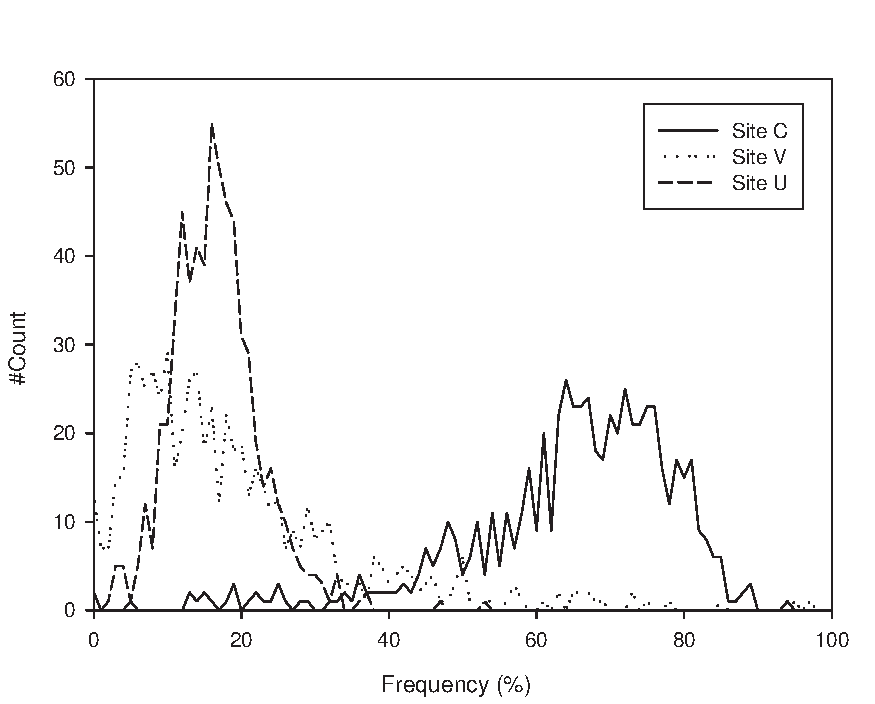
\includegraphics[height=6cm]{figsamp}
\caption{数据曲线图示例}
\label{fig:sample}
\end{figure}

\subsection{表格}

使用浮动环境 \verb|table| 的示例见表\ref{tab:sample}。
\begin{table}
  \caption{表格示例}
  \label{tab:sample}
  \centering
  \begin{tabular}{lcr}%{|l|c|r|}
    \hline
    求解算法                & 系数矩阵的规模    & 执行时间(秒)  \\
    \hline
    Gauss消去法(直接法)     & Mat1903           &  113.27       \\
    Jacobi点迭代            & Mat1784           &  201.36       \\
    \hline
  \end{tabular}
\end{table}

\subsection{数学公式}

本模板提供的文档类 \verb|csoarticle| 本身默认情况下已经包含了 \verb|amsmath| 和 \verb|amsthm| 宏包,因此可以使用这些宏包中提供的一切命令。带编号的数学公式建议使用 \verb|align| 环境。举例如下:一元二次方程
\begin{align}\label{eq:sample}
    a x^2 + b x + c = 0
\end{align}
的两个根为
\begin{align}\label{eq:root}
    x_1 &= \frac{-b + \sqrt{b^2 - 4ac}}{2a} \\
    x_2 &= \frac{-b - \sqrt{b^2 - 4ac}}{2a}
\end{align}
其中,方程\eqref{eq:sample}中的系数$a \not= 0$。

数学类内容中常用的定理类环境也可以直接使用,举例如下(\emph{均为虚拟例子,切勿进行技术性探究}):
\begin{lemma}\label{lem:levy}
    引理的具体内容。
\end{lemma}
\begin{proof}
    可参看各类数学分析类教材,此处从略。
\end{proof}

\begin{theorem}[牛顿第二定律]\label{thm:newton}
物体的质量$m$、物体所受的力$F$以及物体运动的加速度$a$之间满足
\begin{align}\label{eq:f-eq-ma}
    F = m a
\end{align}
\end{theorem}
\begin{proof}
由引理\ref{lem:levy}及文献\cite{bib1}第15章的定理4可立得。
\end{proof}

请直接查看以上例子的源代码部分。

\subsection{参考文献的格式要求}

文献数量应不低于6篇,综述文章文献数量不低于25篇。

注:文中所引的参考文献, 作者均应认真阅读过, 对文献的作者、题目、发表的刊物、年份、卷期号和起止页码等均应核实无误,并按在正文出现的先后顺序编号。标引的序号两边加“[ ]”,作者不超过3人的姓名都写, 超过3人的第三人后面加“,等(et al)” 。无论中外署名,一律姓(大写)先名后,作者姓名之间以逗号分隔。参考文献一律置于文末。文献正文中所有非英文文献需写出对应的英文译文,具体格式要求如下(例子请参看本模板文后的参考文献):
\begin{enumerate}
\item\textbf{期刊:}     作者. 论文题目[J]. 刊名,年,卷(期):起始页码~终止页码.
\item\textbf{专著:}     作者. 书名[M]. 出版地:出版社,出版年.
\item\textbf{译著:}     作者. 书名[M]. 译者. 出版地:出版社,出版年.
\item\textbf{论文集:}   作者. 论文题目[A]. 编者. 文集[C]. 出版地:出版社,出版年. 起始页码~终止页码.
\item\textbf{学位论文:} 作者. 论文题目[D]. 所在城市:保存单位,年份.
\item\textbf{技术标准:} 起草责任者,技术标准代号顺序号—发布年. 技术标准名称[S]. 出版地:出版社,出版年.其中,起草责任者、出版地、出版社、出版年可省。
\item\textbf{专利:}     申请者. 专利名[P]. 国名及专利号,发布日期.
\item\textbf{技术报告:} 作者. 文题[R]. 地名:责任单位,报告代码及编号,年份.
\item\textbf{报纸文章:} 作者. 文题[N]. 报纸名,出版日期(版次).
\item\textbf{在线文献:} 作者. 文题[OL]. [日期]. http://......
\item\textbf{光盘文献:} 作者. 文题[CD]. 出版地:出版者,出版日期.
\item\textbf{其他文献:} 作者. 文题[Z]. 出版地:出版者,出版日期.
\end{enumerate}

\section{结论}

本文给出了………

\section*{致谢(可选)}

应向对论文有帮助的有关人士或单位表示谢意。


%----------------------------------------------------------
% 3. 参考文献
%----------------------------------------------------------

\begin{thebibliography}{2} % 这里的2是指参考文献总数目,需要根据实际情况进行修改
    \bibitem{bib1} H.E.S.Said, T.Tan and K.Baker.Personal identification based on handwriting [J].Pattern Recognition, 33:149-160, Jan. 2000
    \bibitem{bib2} 吴佑寿,丁晓青.汉字识别原理与应用[M],北京:高等教育出版社,1992.8
\end{thebibliography}

\end{document}
